\section{实验目的}

本实验围绕亚洲人脸的颜色与几何结构分割任务，研究如何利用颜色统计与五官几何先验从图像中准确分割脸部区域。首先从带有像素级标签的训练图像中提取肤色样本，统计其在颜色空间中的分布；再以统计参数构造颜色候选，结合连通域与形态学处理恢复包含眼睛、眉毛和嘴部的脸部区域；进而引入灰度黑帽双眼定位、内外嵌套双椭圆空间约束、侧向姿态椭圆候选与低支持放宽肤色阈值重建，系统检验各模块对分割准确度的提升作用。

\section{相关原理与数据准备}
\subsection{颜色空间与分割原理}

直接使用 RGB 三个通道描述肤色时，亮度和颜色信息混合在一起。YCrCb 将亮度信息主要表示在 Y 通道中，并使用 Cr、Cb 两个色差通道描述颜色，为单独研究肤色的颜色分布提供了方便。实验三使用 Cr、Cb 建立肤色统计，Y 不参与颜色范围的估计；实验四则在颜色模型基础上进一步结合灰度通道提取眼部暗斑几何特征。

实现中以 8 位 BGR 顺序读取原图，使用 OpenCV 的 \texttt{COLOR\_BGR2YCrCb} 转换，输出通道顺序为 Y、Cr、Cb，编码值范围为 0--255。图像保持原始尺寸和颜色，不做缩放、白平衡或颜色增强；后续分割沿用相同处理方式，使统计参数与待分割像素处于一致的表示中。

颜色分割的依据是：训练肤色在 Cr/Cb 平面中存在较集中的分布区域，可用均值和标准差概括其位置与离散程度，为候选区域的判定提供参数。由于具有相近颜色的头发、脖颈或背景也可能被选中，而眼睛和嘴部又可能不满足肤色范围，颜色筛选提供的是初始候选像素，完整脸部还需要结合空间结构与几何先验处理。

\subsection{数据来源与集合划分}

实验使用 Face\_segment 数据集及其原始多类别像素标签。从原数据的 \path{test/real_image/2} 目录中筛选出符合亚洲人脸特征的样本，并保留对应原始标签。最初选入 163 对图像与标签；程序核对了图像与标签的配对关系、尺寸及标签取值，发现 00583 与 00584 的图像文件完全相同，经核对保留 00583、剔除 00584，最终得到 162 对有效数据。原图均为 $512\times512$ 的 RGB 图像，标签为单通道类别图，包含 0--18 的原始类别编码。通过原图、彩色标签和半透明叠加图逐张核查后，确认图像与标签配对准确。

在此基础上，将样本编号排序后以固定随机种子 42 打乱，按约 $6:2:2$ 划分为表~\ref{tab:datasplit} 中的三个集合，并通过 64 位感知哈希（dHash）筛查确认集合间不存在同一照片裁剪或缩放重复。

\begin{table}[H]
\centering
\small
\caption{数据集的固定划分与用途}\label{tab:datasplit}
\begin{tabular}{lrl}
\toprule
集合 & 图像数量 & 用途 \\
\midrule
训练集 & 98 & 提取肤色像素与五官坐标，计算颜色统计参数与椭圆几何先验 \\
验证集 & 32 & 比较阈值系数、后处理方案及双椭圆形态学消融实验 \\
测试集 & 32 & 评价基础颜色分割方案的泛化表现 \\
\bottomrule
\end{tabular}
\end{table}

\subsection{标签定义与肤色样本提取}\label{sec:labeldefinition}

本实验区分肤色建模区域与完整脸部评价区域。前者用于估计颜色参数，只选取皮肤和鼻子；后者用于评价分割是否覆盖整张脸部，需要纳入双眼、双眉和嘴部。原始标签保持不变，按表~\ref{tab:labelmapping} 的规则分别提取统计像素和生成评价真值。

\begin{table}[H]
\centering
\small
\caption{原始标签在颜色统计与脸部评价中的用途}\label{tab:labelmapping}
\begin{tabularx}{\textwidth}{l l X}
\toprule
用途 & 标签编号 & 对应区域 \\
\midrule
肤色统计 & 1、2 & 皮肤、鼻子 \\
脸部评价正类 & 1、2、4--7、10--12 & 皮肤、鼻子、双眼、双眉、口腔、上下唇 \\
评价忽略区域 & 3 & 眼镜 \\
脸部评价负类 & 其余类别 & 背景、双耳、头发、帽子、饰品、脖颈和衣服等 \\
\bottomrule
\end{tabularx}
\end{table}

眼睛、眉毛和嘴部属于最终分割目标，但其颜色通常偏离皮肤；若将它们一并用于肤色建模，会干扰肤色分布统计。因此，这些区域不参与肤色参数计算，后续通过连通域填孔与形态学修补恢复其覆盖。眼镜区域设为忽略类别，不计入混淆计数。

\begin{figure}[htbp]
\centering
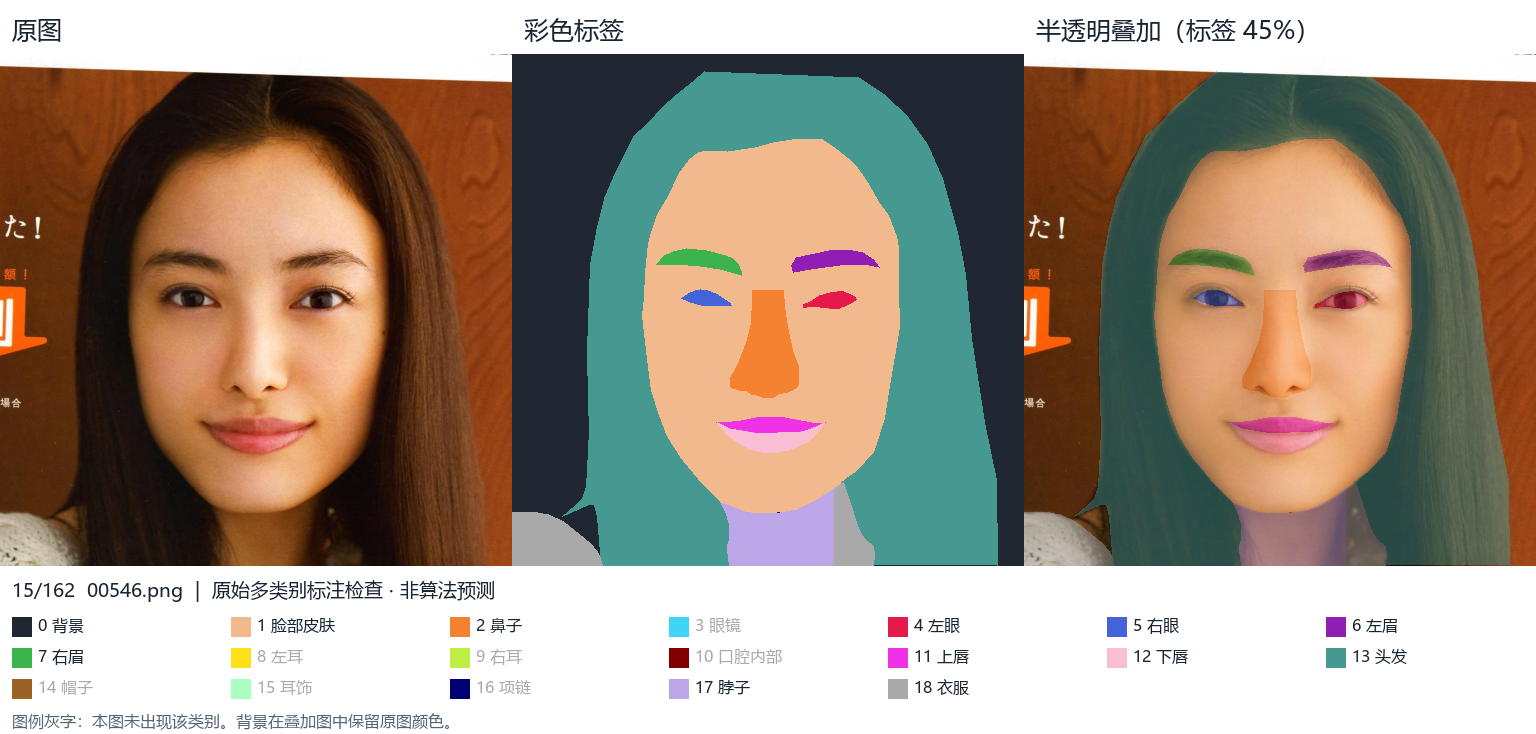
\includegraphics[width=\textwidth]{part_a_label_review_00546.png}
\caption{样本 00546 的原图、原始多类别标签及叠加核查图。}
\label{fig:partalabel}
\end{figure}

图~\ref{fig:partalabel} 展示了原始标签对皮肤、鼻子、眼睛、眉毛和嘴部的区分，也显示头发和脖颈虽与脸部相邻，但在评测中属于负类。明确这些边界后，后续评价才能区分脸部内部缺失与脸部外部误检。
\FloatBarrier

\subsection{训练肤色统计}

从 98 张训练图中共提取皮肤像素 5,838,561 个、鼻子像素 548,991 个，合计 $N=6{,}387{,}552$ 个。所有选中像素等权汇总，计算训练集全部选中肤色像素的总体均值、总体方差与标准差：
\begin{equation}
\mu_c=\frac{1}{N}\sum_{i=1}^{N}c_i,\qquad
\sigma_c^2=\frac{1}{N}\sum_{i=1}^{N}(c_i-\mu_c)^2,\qquad
\sigma_c=\sqrt{\sigma_c^2},\qquad c\in\{Cr,Cb\}.
\label{eq:skinstatistics}
\end{equation}
计算结果如表~\ref{tab:skinparams} 所示。

\begin{table}[H]
\centering
\small
\caption{训练集皮肤与鼻子像素的颜色统计参数}\label{tab:skinparams}
\begin{tabular}{lrrr}
\toprule
通道 & 均值 & 总体方差 & 标准差 \\
\midrule
Cr & 151.14949561 & 87.88095189 & 9.37448409 \\
Cb & 109.11018055 & 89.93800609 & 9.48356505 \\
\bottomrule
\end{tabular}
\end{table}

\begin{figure}[htbp]
\centering
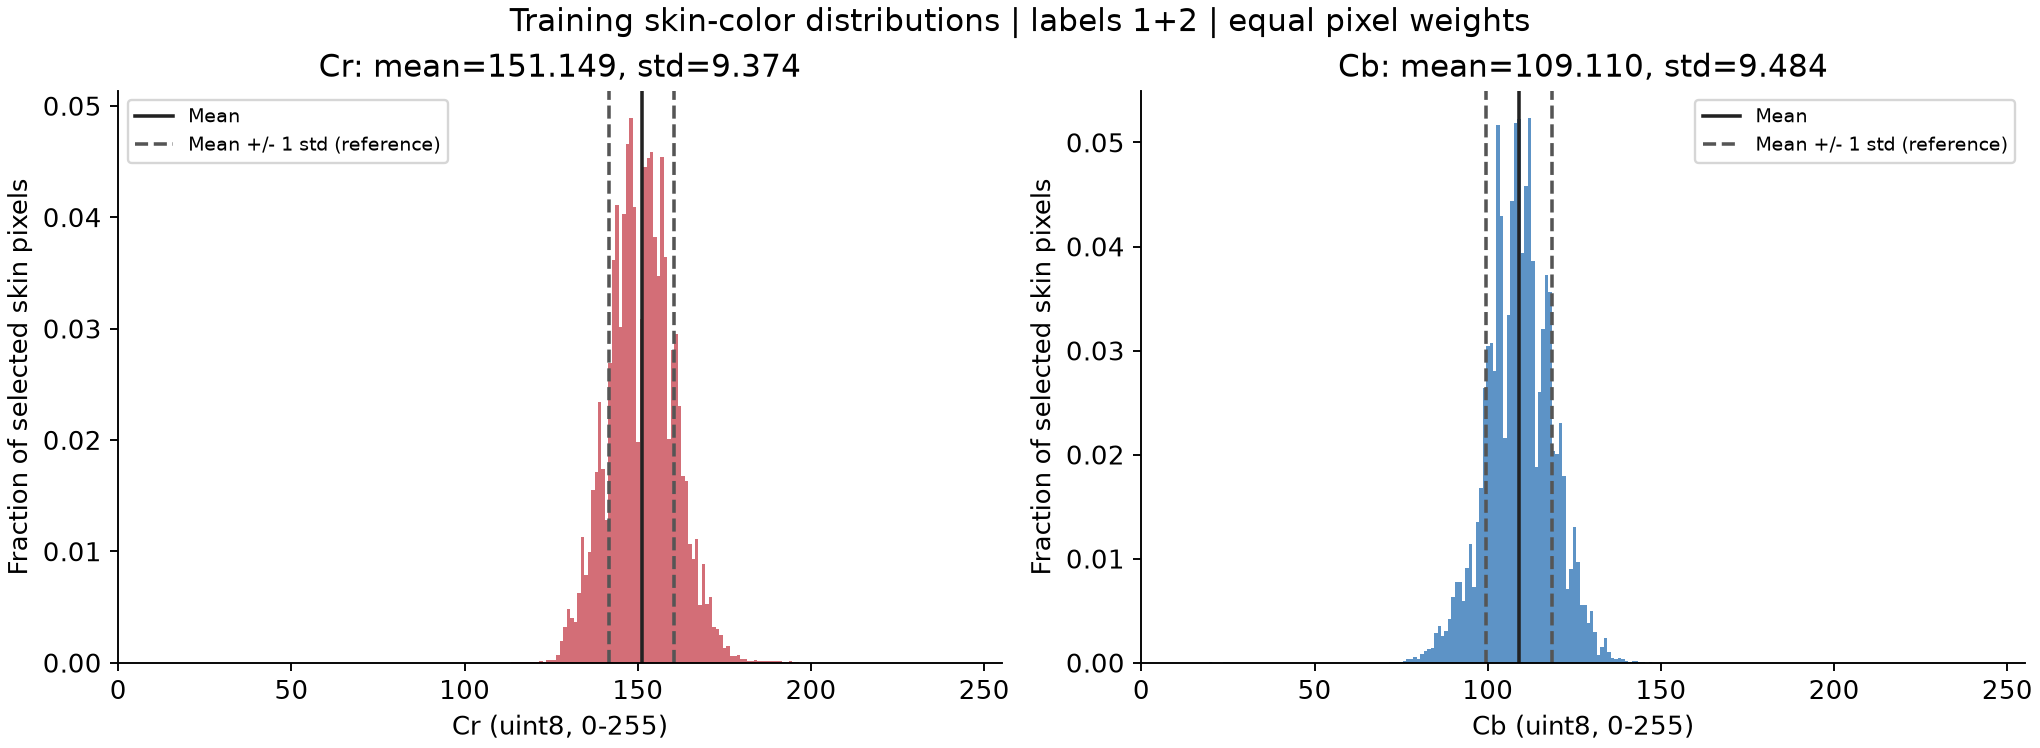
\includegraphics[width=\textwidth]{part_a_channel_distributions.png}
\caption{训练肤色像素的 Cr、Cb 单通道分布（实线表示均值，虚线表示均值加减一个标准差）。}
\label{fig:partachannels}
\end{figure}

图~\ref{fig:partachannels} 中，两通道均存在明显的单峰集中区域，主要像素分布在均值附近，两通道标准差均约为 9.4 个编码值。

\begin{figure}[htbp]
\centering
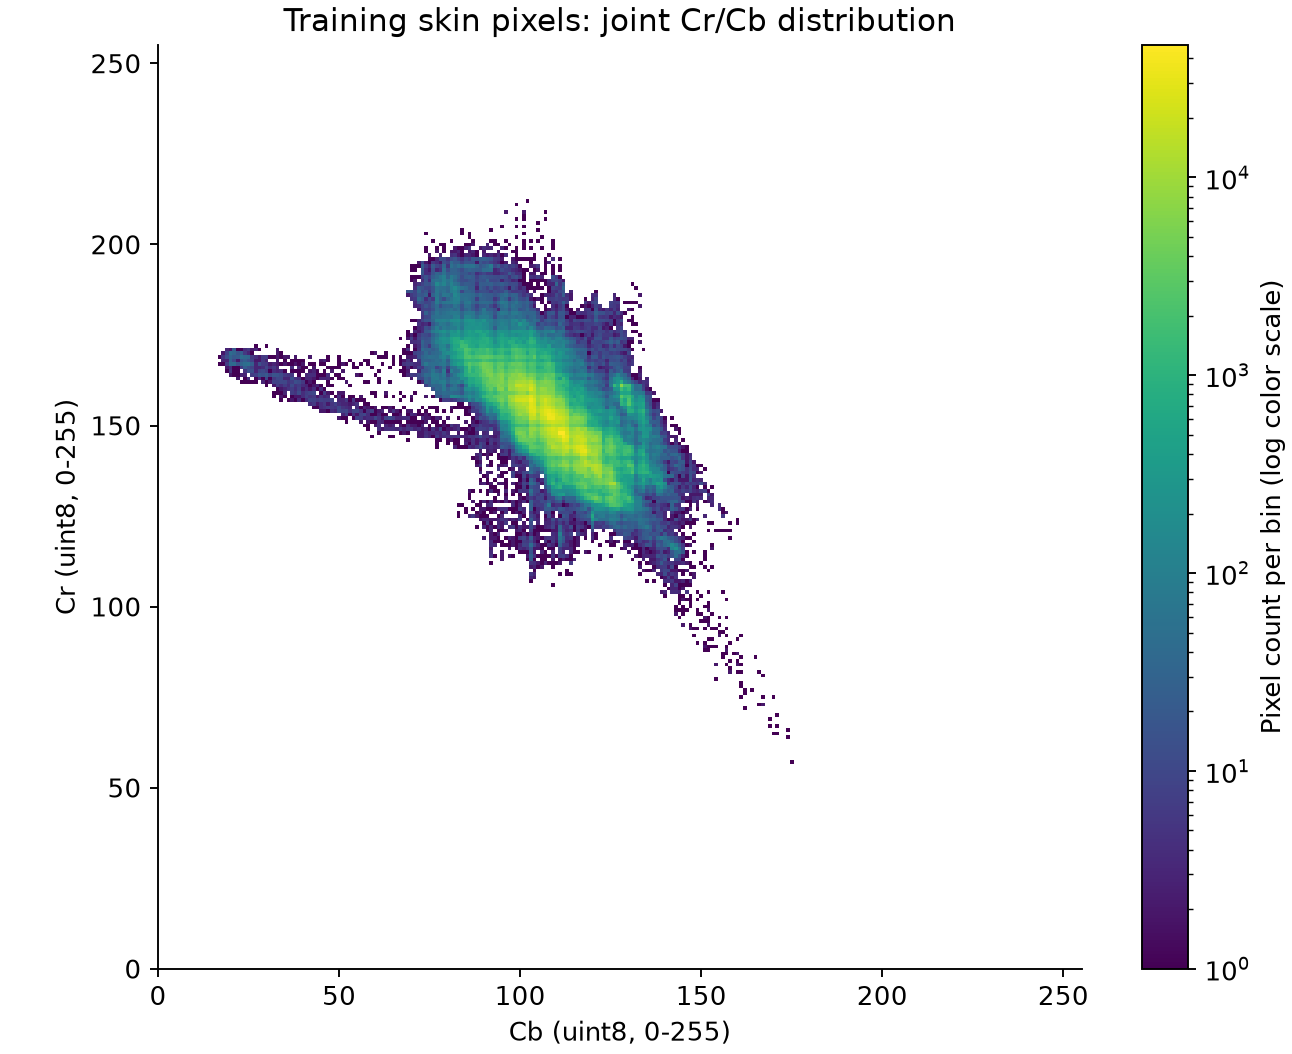
\includegraphics[width=0.73\textwidth]{part_a_joint_distribution.png}
\caption{训练肤色像素的 Cr/Cb 联合分布（对数频数刻度）。}
\label{fig:partajoint}
\end{figure}

联合分布进一步揭示了两个通道之间的相关性。图~\ref{fig:partajoint} 的高频区域整体呈倾斜椭圆形状，按像素频数计算的相关系数约为 $-0.7644$，表明 Cr 较大的像素往往对应较小的 Cb。分别限制 Cr 和 Cb 的上下界得到的是轴对齐矩形：范围过宽可能纳入角落处的非肤色像素，范围过窄又可能漏掉沿倾斜方向延伸的肤色，因此需要结合验证集选择合理的阈值系数 $k$ 与空间后处理策略。
\FloatBarrier
